การทำนายตำแหน่งถัดไปของวัตถุ\textsuperscript{\cite{danelljan2014accurate}} คือระบบที่ใช้สำหรับการติดตามการเคลื่อนไหวของวัตถุที่สนใจที่อยู่ในรูปภาพ 
โดยใช้การคำนวณทางคณิตศาสตร์ และการประมวลผลภาพ (image processing) ทำให้การประมวลผลนั้นเร็วกว่าการใช้โมเดลปัญญาประดิษฐ์

\begin{figure}[!ht]
	\centering
	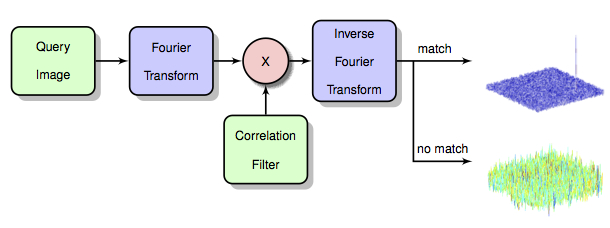
\includegraphics[width=1\textwidth]{chapter2/images/track-concept.png}
		\caption{แนวคิดของระบบทำนายตำแหน่งถัดไปของวัตถุ}
    	\label{fig:Track_concept}
\end{figure}

จากรูปที่ \ref{fig:Track_concept} เป็นหลักการในการทำนายตำแหน่งต่อไป [feihong this way] โดยการนำรูปมาผ่านกระบวนการแปลงฟูรีเยร์ (fourier transform)
และนำมาคูณกับ correlation filter ซึ่งเป็นตัวกรองที่ใช้สำหรับการหาความสัมพันธ์กับวัตถุในภาพ จากนั้นทำการแปลงฟูรีเยร์ผกผัน (inverse fourier transform) 
เพื่อตรวจสอบว่าวัตถุในภาพนั้นอยู่ที่ตำแหน่งใด โดยมีการคำนวณเริ่มจากการหา correlation filter ที่ดีที่สุดโดยใช้วิธีลดผลรวมของข้อผิดพลาดกำลังสองให้น้อยที่สุดดังนี้

\begin{equation}
\epsilon = \left \| \sum_{l = 1}^{d} h^{l} \star f^{l} - g \right \| + \lambda \sum_{l = 1}^{d}\left \| h^{l} \right \|^2
\end{equation}
โดยที่
\begin{conditions}
 \epsilon     	&   ค่าความคลาดเคลื่อน 							\\
 d      		&  จำนวนมิติของผังคุณลักษณะ (feature map) ของภาพ  \\   
 h 			&  correlation filter								\\
\star 			&  circular correlation							\\
 f			&  พื้นที่สี่เหลี่ยมของวัตถุที่สนใจที่ได้จากการทำผังคุณลักษณะ	\\
 g			&  ผลลัพธ์ correlation ที่ต้องการของ f					\\
 \lambda   		&  regularization term
\end{conditions}

เมื่อพิจารณาจากรูปภาพเดียวในกรณีที่เวลา ($t$) เท่ากับ 1 จะสามารถจัดรูปสมการด้านบนได้ดังนี้ 

\begin{equation}
H^{l} = \frac{\bar{G}F^{l}}{\sum_{k=1}^{d}\bar{F^{k}}F^{k} + \lambda}
\end{equation}
\begin{equation}
H_{t}^{l} = \frac{A_{t}^{l}}{B_{t}}					
\end{equation}					
\begin{equation}
A_{t}^{l} = (1-\eta )A_{t-1}^{l} + \eta \bar{G_{t}}F_{t}^{l}
\end{equation}
\begin{equation}
B_{t} = (1-\eta )B_{t-1} + \eta \sum_{k=1}^{d}\bar{F_{t}^{k}}F_{t}^{k}
\end{equation}
โดยที่
\begin{conditions}
 H 		     	&   correlation filter								\\
 \eta      		&  อัตราการเรียนรู้						 		\\   
 \bar{G} 		&  คือ g ที่ผ่านการทำ complex conjugation				\\
 F			&  พื้นที่สี่เหลี่ยมของวัตถุที่สนใจที่ได้จากการทำผังคุณลักษณะ	\\
 \bar{F}		&   f ที่ผ่านการทำ complex conjugation					\\
 t 	  		&  เวลา
\end{conditions}
จากสมการที่ได้มาจะสามารถทำให้หาตำแหน่งต่อไปของวัตถุที่สนใจได้ด้วยสมการต่อไปนี้
\begin{equation}
y = F^{-1}\left \{ \frac{\sum_{l = 1}^{d} \bar{A^{l}}Z^{l}}{B + \lambda} \right \}
\end{equation}
โดยที่
\begin{conditions}
 y 		     	&   correlation score										\\
 F^{-1}    		&  การแปลงฟูรีเยร์ผกผันแบบไม่ต่อเนื่อง (inverse discrete fourier transform)						\\   	
 Z	 		&  พื้นที่สี่เหลี่ยมของวัตถุที่สนใจที่ได้จากการหาผังคุณลักษณะของภาพใหม่	
\end{conditions}
โดยค่าของ $y$ ที่ได้ออกมาจะทำให้รู้ถึงตำแหน่งของวัตถุที่สนใจได้ ณ ตำแหน่งที่ $y$ มีค่าสูงสุด